\documentclass{article}
\usepackage{graphicx}
\usepackage{amsmath}
\usepackage{listings}
\usepackage{hyperref}
\usepackage{float}
\usepackage{xcolor}    % For syntax highlighting
\usepackage{listings}
%
% Enhanced listing settings
\lstset{
    basicstyle=\ttfamily\footnotesize,
    breaklines=true,
    frame=single,
    captionpos=b,
    tabsize=4,
    commentstyle=\color{green!60!black},
    keywordstyle=\color{blue},
    stringstyle=\color{red},
    numberstyle=\tiny,
    numbersep=5pt
}

\title{Mini-Project: Sorting Algorithms}
\author{HADJ ARAB Adel \and BECHAR Walid}
\date{\today}

\begin{document}

\maketitle

\section{Introduction}
Sorting is one of the most classically studied families of algorithms, because they are among the modules essential for the good running of more advanced algorithms. The general principle of a sorting algorithm is to order (in ascending order for example) the objects of a collection of data (values), according to a comparison criterion (key – for us, values and keys are here confused: these are the elements of an array of integers). We generally carry out sorting by using an "in-place" approach: the sorted values are stored in the same array as the initial values (which therefore becomes an input-output parameter).

\section{Sorting Algorithms}

\subsection{Bubble Sort}

\subsubsection{Algorithm}
The \textbf{Bubble Sort} function in C sorts an array of integers in ascending order using the bubble sort algorithm. It iterates through the array multiple times, comparing and swapping adjacent elements if they are in the wrong order. The process is repeated until the array is sorted. An optimization is included with a \textbf{change flag} that allows the function to exit early if no swaps are made during a pass, indicating that the array is already sorted. This reduces unnecessary iterations and improves efficiency.

\newpage
\begin{lstlisting}[language=C, caption=Bubble Sort implementation]
void bubble_sort(int arr[], int n) {
  int change = 1; // boolean variable
  while (change) {
    change = 0;
    for (int i = 0; i < n - 1; i++) {
      if (arr[i] > arr[i + 1]) {
        swap(&arr[i], &arr[i + 1]);
        change = 1;
      }
    }
  }
}
\end{lstlisting}

The \textbf{Optimized Bubble Sort} function in C sorts an array of integers in ascending order using an optimized version of the bubble sort algorithm. It iterates through the array multiple times, comparing and swapping adjacent elements if they are in the wrong order. The process is repeated until the array is sorted. An optimization is included with a \textbf{change flag} that allows the function to exit early if no swaps are made during a pass, indicating that the array is already sorted. Additionally, the range of the inner loop is reduced by one after each pass, as the largest elements are moved to their correct positions at the end of the array. This reduces unnecessary comparisons and improves efficiency.

\begin{lstlisting}[language=C, caption=Optimized Bubble Sort implementation]
void optimized_bubble_sort(int arr[], int n) {
  int m = n - 1;
  int change = 1;

  while (change) {
    change = 0;
    for (int i = 0; i < m; i++) {
      if (arr[i] > arr[i + 1]) {
        swap(&arr[i], &arr[i + 1]);
        change = 1;
      }
    }
    m--;
  }
}
\end{lstlisting}

\newpage
\subsubsection{Complexity}
Both Bubble Sort and Optimized Bubble Sort have a worst-case and average-case time complexity of $O(n^2)$, where $n$ is the number of elements to be sorted. This is because, in the worst case, each element needs to be compared with every other element, resulting in $n(n-1)/2$ comparisons.

However, the best-case time complexity differs between the two algorithms. For Bubble Sort, the best-case time complexity is $O(n)$ when the array is already sorted, as the algorithm will still iterate through the entire array once to confirm that no swaps are needed. For Optimized Bubble Sort, the best-case time complexity is also $O(n)$, but it can potentially reduce the number of comparisons further due to the decreasing range of the inner loop after each pass.

The space complexity for both algorithms is $O(1)$ as they are in-place sorting algorithms, meaning they do not require additional memory proportional to the input size.

\subsubsection{Results}
\begin{figure}[H]
	% \centering
	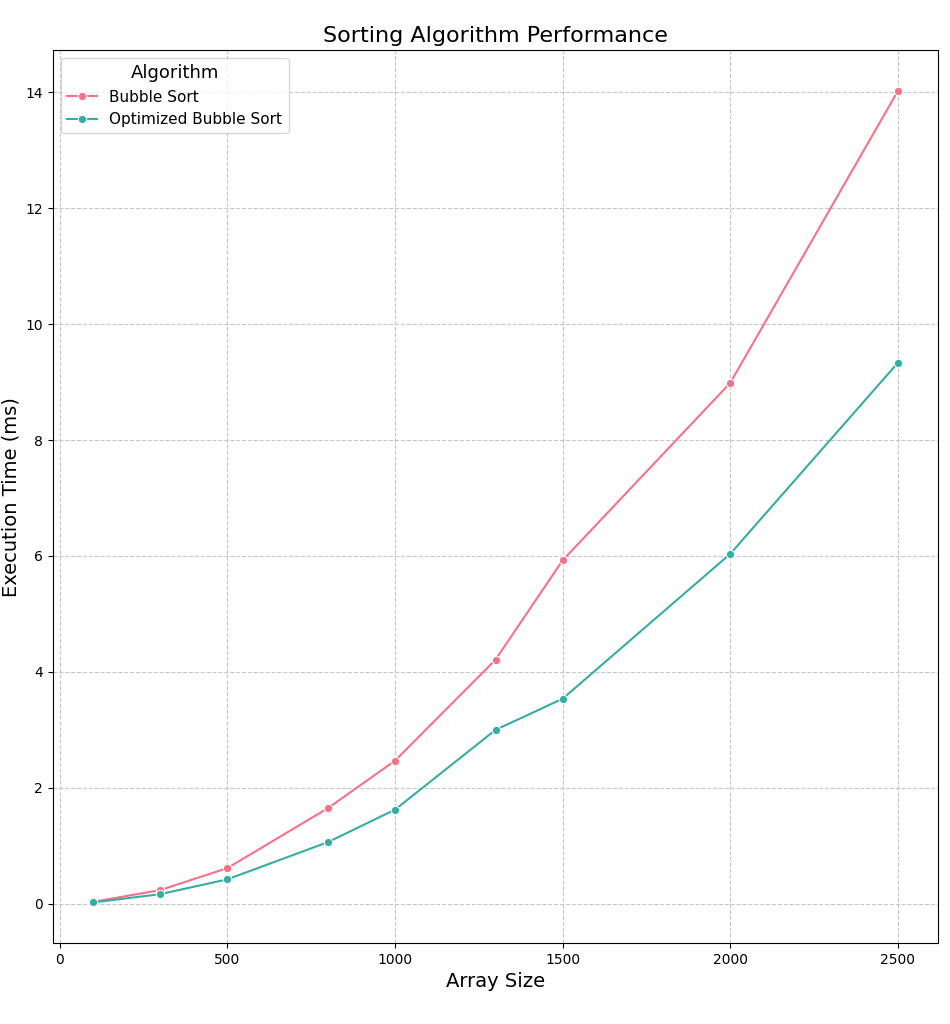
\includegraphics[width=0.8\textwidth]{images/bubble_sort_comparaison.png}
	\caption{Bubble Sort and Optimized Bubble Sort running time as a function of $n$}
\end{figure}


\subsection{Gnome Sort}

\subsubsection{Algorithm}
The \textbf{Gnome Sort} function in C sorts an array of integers in ascending order by iteratively comparing each element with the next one and swapping them if they are out of order, moving the index backward after a swap to recheck previous elements, and moving it forward otherwise, continuing this process until the entire array is sorted, ensuring that each element is in its correct position by the end of the algorithm.

\begin{lstlisting}[language=C, caption=Gnome Sort implementation]
void gnome_sort(int arr[], int n) {
  int i = 0;

  while (i < n - 1) {
    if (arr[i] <= arr[i + 1]) {
      i++;
    } else {
      swap(&arr[i], &arr[i + 1]);
      if (i > 0) {
        i--;
      } else {
        i++;
      }
    }
  }
}
\end{lstlisting}

\subsubsection{Complexity}
Gnome Sort has a worst-case and average-case time complexity of $O(n^2)$, where $n$ is the number of elements to be sorted. The best-case time complexity is $O(n)$ when the array is already sorted. The space complexity is $O(1)$ as it is an in-place sorting algorithm.

\subsubsection{Results}
\begin{figure}[H]
	% \centering
	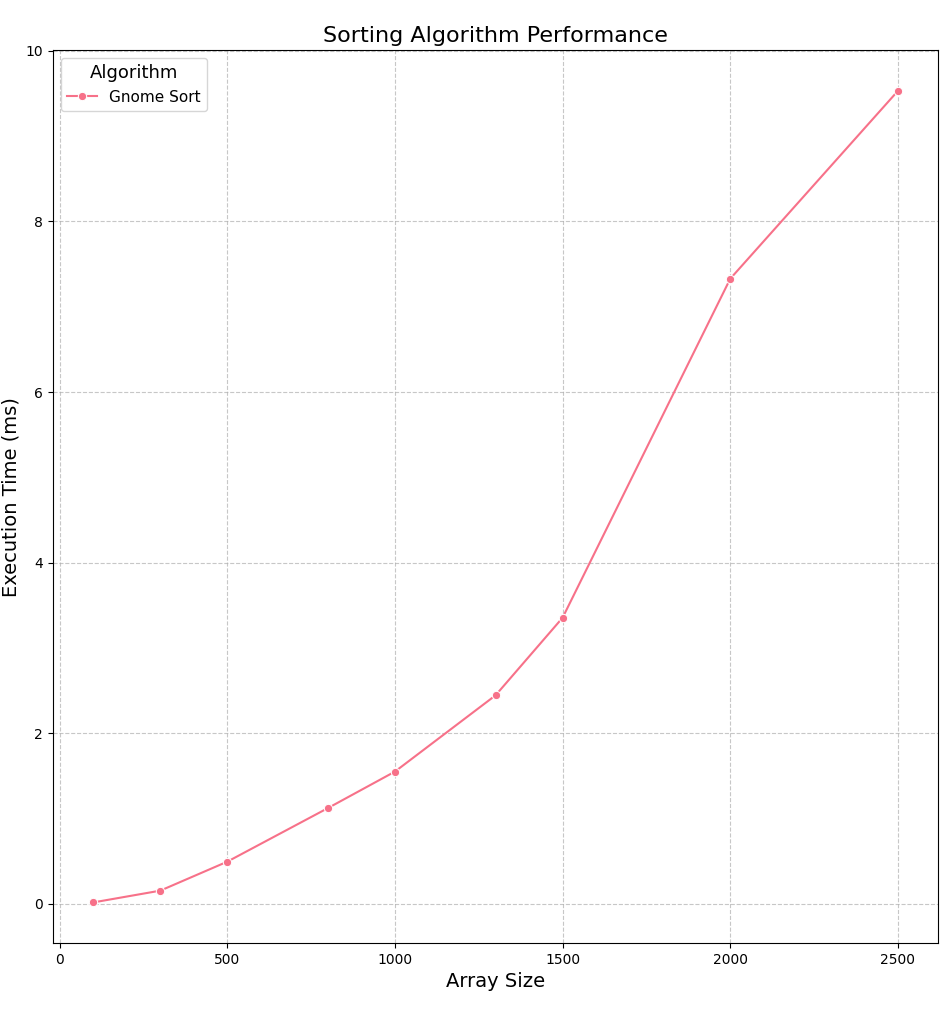
\includegraphics[width=0.8\textwidth]{images/gnome_sort.png}
	\caption{Gnome Sort running time as a function of $n$}
\end{figure}


\subsection{Radix Sort}

\subsubsection{Algorithm}
The \textbf{Sort Aux} function in C sorts an array of integers based on a specific digit (determined by the parameter `i`) using a counting sort approach, where it first counts the occurrences of each digit, then calculates the cumulative count, places the elements into an output array in sorted order according to the current digit, and finally copies the sorted elements back into the original array, ensuring that the array is partially sorted by the specified digit.

\newpage
\begin{lstlisting}[language=C, caption=Sort Aux implementation]
void sort_aux(int arr[], int n, int i) {
  int *output = (int *)malloc(n * sizeof(int));
  int count[10] = {0};

  for (int j = 0; j < n; j++) {
    count[key(arr[j], i)]++;
  }
  for (int j = 1; j < 10; j++) {
    count[j] += count[j - 1];
  }
  for (int j = n - 1; j >= 0; j--) {
    output[count[key(arr[j], i)] - 1] = arr[j];
    count[key(arr[j], i)]--;
  }
  for (int j = 0; j < n; j++) {
    arr[j] = output[j];
  }

  free(output);
}
\end{lstlisting}

The \textbf{Radix Sort Helper} function in C sorts an array of integers by iterating through each digit from the least significant to the most significant, calling the \textbf{Sort Aux} function to sort the array based on the current digit, while the \textbf{Radix Sort} function determines the maximum number of digits in the largest number of the array and then calls \textbf{Radix Sort Helper} to perform the sorting process, ensuring the entire array is sorted by all digits.

\begin{lstlisting}[language=C, caption=Radix Sort implementation]
void radix_sort_helper(int arr[], int n, int k) {
  // k represents the maximum number of digits
  for (int i = 0; i < k; i++) {
    sort_aux(arr, n, i);
  }
}

void radix_sort(int arr[], int n) {
  // maximum number of digits is the number of digits of the largest number
  int imax = 0;
  for (int i = 1; i < n; i++) {
    if (arr[i] > arr[imax]) {
      imax = i;
    }
  }

  int k = (int)log10(arr[imax]) + 1;
  radix_sort_helper(arr, n, k);
}
\end{lstlisting}

\subsubsection{Complexity}
Radix Sort has a time complexity of $O(d \cdot (n + k))$, where $d$ is the number of digits in the largest number, $n$ is the number of elements, and $k$ is the range of the digit values. The space complexity is $O(n + k)$.

\subsubsection{Results}
\begin{figure}[H]
	% \centering
	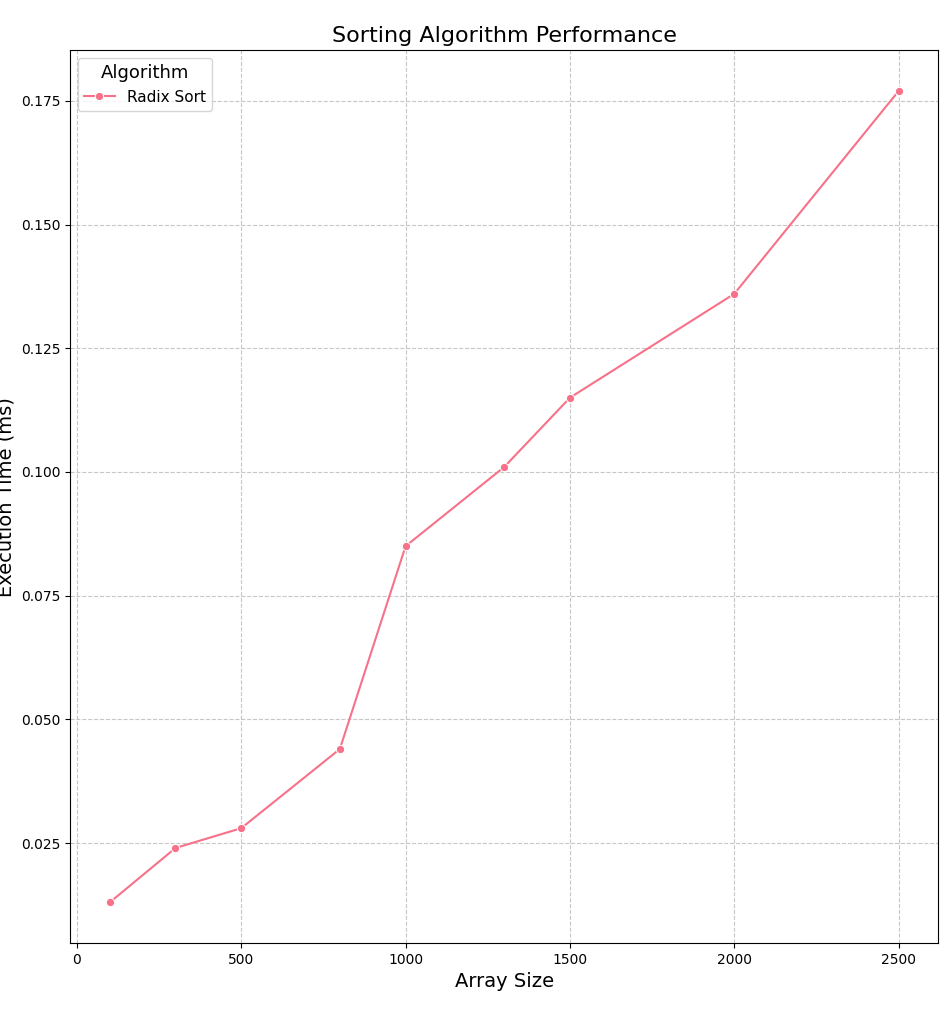
\includegraphics[width=0.8\textwidth]{images/radix_sort.png}
	\caption{Radix Sort running time as a function of $n$}
\end{figure}


\subsection{Quick Sort}

\subsubsection{Algorithm}
The \textbf{Partition} function in C rearranges the elements of an array around a pivot element (chosen as the first element of the array segment) such that all elements less than or equal to the pivot are on its left and all elements greater than the pivot are on its right, by iteratively moving indices from both ends towards the center, swapping elements as needed, and finally placing the pivot in its correct position, returning the index of the pivot.

\begin{lstlisting}[language=C, caption=Partition implementation]
int partition(int arr[], int low, int high) {
  int p = arr[low];
  int i = low;
  int j = high;

  while (i < j) {
    while (arr[i] <= p && i <= high - 1) {
      i++;
    }
    while (arr[j] > p && j >= low + 1) {
      j--;
    }
    if (i < j) {
      swap(&arr[i], &arr[j]);
    }
  }
  swap(&arr[low], &arr[j]);
  return j;
}
\end{lstlisting}

The \textbf{Quick Sort Helper} function in C recursively sorts an array of integers by partitioning the array around a pivot element and then sorting the subarrays on either side of the pivot, while the \textbf{Quick Sort} function serves as a wrapper that initializes the recursive process by calling \textbf{Quick Sort Helper} with the full range of the array.

\begin{lstlisting}[language=C, caption=Quick Sort implementation]
void quick_sort_helper(int arr[], int low, int high) {
  if (low < high) {
    int pi = partition(arr, low, high);

    quick_sort_helper(arr, low, pi - 1);
    quick_sort_helper(arr, pi + 1, high);
  }
}

void quick_sort(int arr[], int n) { quick_sort_helper(arr, 0, n - 1); }
\end{lstlisting}

\subsubsection{Complexity}
Quick Sort has a worst-case time complexity of $O(n^2)$, which occurs when the pivot selection is poor. However, the average-case and best-case time complexity is $O(n \log n)$. The space complexity is $O(\log n)$ due to the recursive stack space.

\subsubsection{Results}
\begin{figure}[H]
	% \centering
	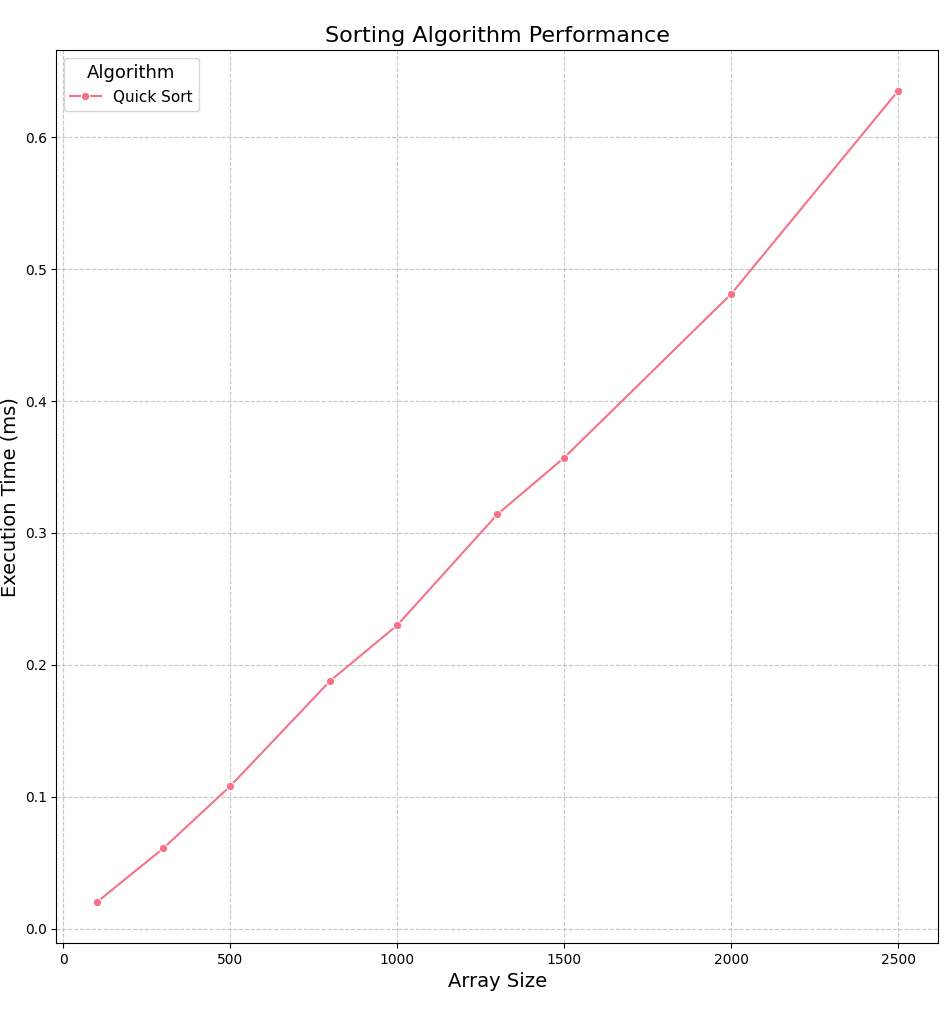
\includegraphics[width=0.8\textwidth]{images/quick_sort.png}
	\caption{Quick Sort running time as a function of $n$}
\end{figure}


\subsection{Heap Sort}

\subsubsection{Algorithm}
The \textbf{Heapify} function in C maintains the heap property of a binary heap by comparing a node with its children and swapping it with the largest child if necessary, then recursively applying the same process to the affected subtree, ensuring that the subtree rooted at the given node becomes a valid max-heap.

\newpage
\begin{lstlisting}[language=C, caption=Heapify implementation]
void heapify(int arr[], int n, int i) {
  int largest = i;
  int left = 2 * i + 1;  // Left child
  int right = 2 * i + 2; // Right child

  if (left < n && arr[left] > arr[largest])
    largest = left;

  if (right < n && arr[right] > arr[largest])
    largest = right;

  if (largest != i) {
    swap(&arr[i], &arr[largest]);
    heapify(arr, n, largest);
  }
}
\end{lstlisting}

The \textbf{Heap Sort} function in C sorts an array of integers in ascending order by first building a max heap from the array, then repeatedly extracting the maximum element from the heap and placing it at the end of the array, and finally re-heapifying the remaining elements until the entire array is sorted.

\begin{lstlisting}[language=C, caption=Heap Sort implementation]
void heap_sort(int arr[], int n) {
  // Build max heap
  for (int i = n / 2 - 1; i >= 0; i--)
    heapify(arr, n, i);

  // Extract elements from heap one by one
  for (int i = n - 1; i > 0; i--) {
    swap(&arr[0], &arr[i]);
    heapify(arr, i, 0);
  }
}
\end{lstlisting}

\subsubsection{Complexity}
Heap Sort has a time complexity of $O(n \log n)$ for all cases (worst, average, and best). The space complexity is $O(1)$ as it is an in-place sorting algorithm.

\subsubsection{Results}
\begin{figure}[H]
	% \centering
	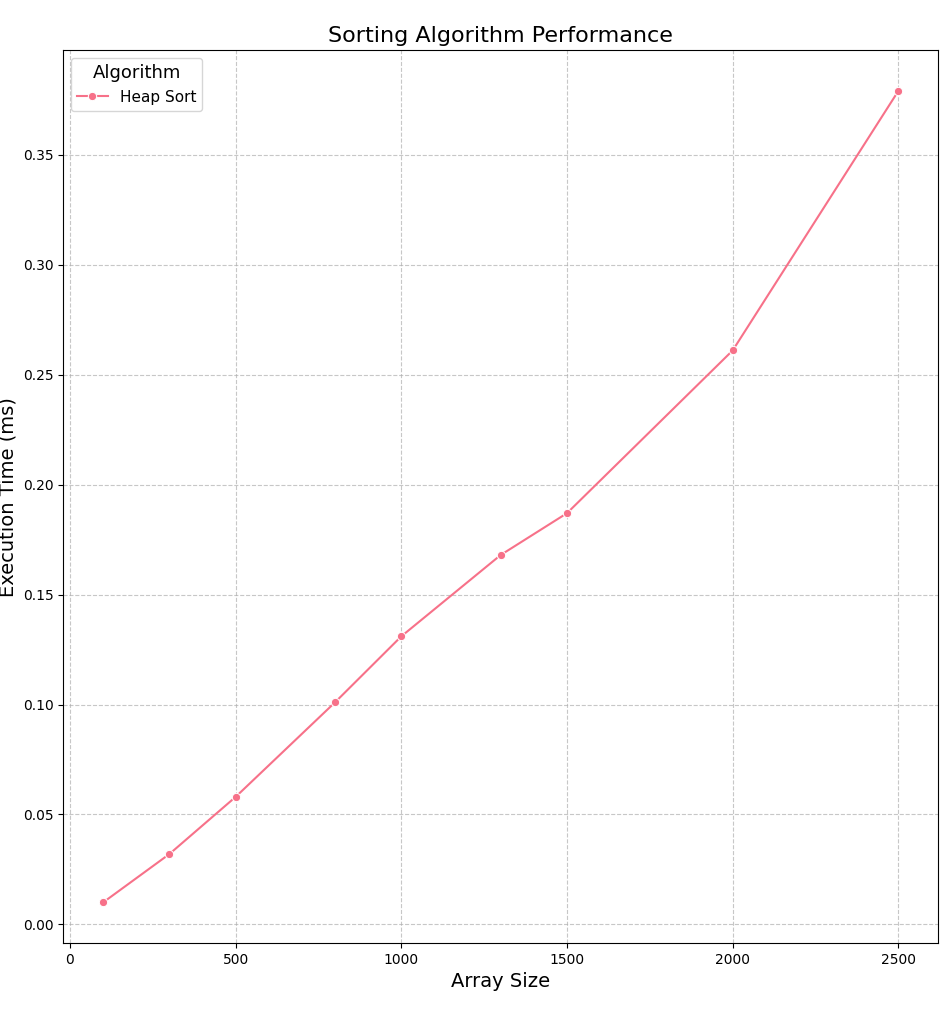
\includegraphics[width=0.8\textwidth]{images/heap_sort.png}
	\caption{Heap Sort running time as a function of $n$}
\end{figure}

\section{Evaluation}
In this section, we conduct a comprehensive evaluation of the performance of the implemented sorting algorithms. We meticulously compare their execution times across a diverse range of input sizes to provide a thorough analysis. This comparison will highlight the efficiency and scalability of each algorithm, offering valuable insights into their practical applications and limitations.

\begin{figure}[H]
	% \centering
	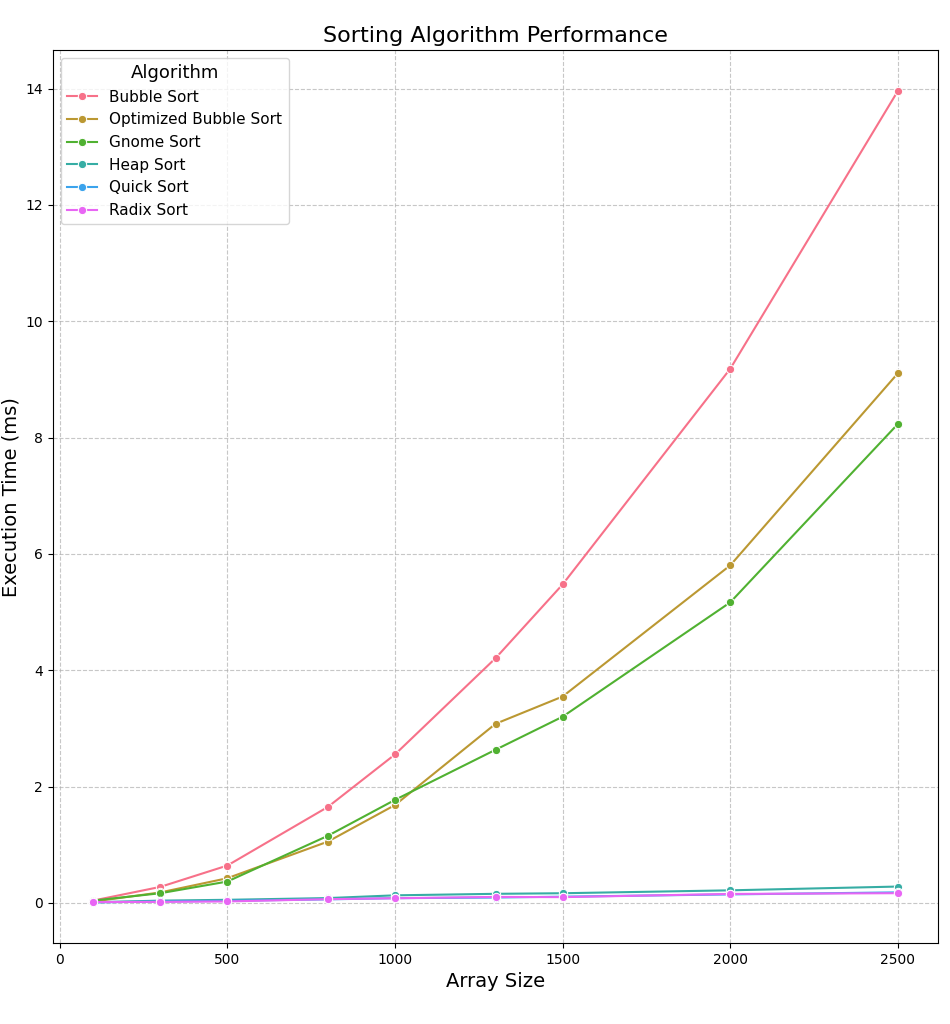
\includegraphics[width=0.8\textwidth]{images/all_sorts.png}
	\caption{All Sorting Algorithms running time as a function of $n$}
\end{figure}

\section{Conclusion}
In this project, we have successfully implemented and rigorously tested a variety of sorting algorithms. Through detailed analysis, we have studied their computational complexities and compared these theoretical complexities with empirical evaluations of their running costs. The experimental results have consistently aligned with our theoretical expectations, thereby validating the efficiency and effectiveness of the sorting algorithms under study. This comprehensive evaluation not only reinforces the theoretical foundations of these algorithms but also provides practical insights into their performance across different scenarios. Our findings underscore the importance of understanding algorithmic complexity and its real-world implications, ultimately contributing to the broader field of computer science and algorithm design.

\end{document}
